\documentclass{article}
\usepackage{cmap}
\usepackage[utf8]{inputenc}
\usepackage[english,ukrainian]{babel}
\usepackage{graphicx}
\usepackage{geometry}
\usepackage{listings}
\usepackage{float}
\usepackage{amsmath}
\geometry{
	a4paper,
	left=20mm,
	right=20mm,
	top=15mm,
	bottom=15mm,
}
\lstset{
	language=c,
	tabsize=4,
	keepspaces,
	showstringspaces=false,
}
\graphicspath{ {./pictures} }
\setlength{\parindent}{4em}

\newcommand\subject{Архітектура комп'ютера}
\newcommand\lecturer{доцент кафедри ПЗ\\Крук О.Г.}
\newcommand\teacher{доцент кафедри ПЗ\\Крук О.Г.}
\newcommand\mygroup{ПЗ-22}
\newcommand\lab{1}
\newcommand\theme{Моделювання логічних елементів в середовищі системи Proteus. Синтез та моделювання простих логічних схем}
\newcommand\purpose{Набути практичних навиків моделювання логічних елементів та схем в середовищі системи програм Proteus; закріпити вміння складати за таблицею істиності логічні функції в досконалій диз'юнктивній та кон'юнктивній нормальній формі; опанувати синтез простих комбінаційних схем за логічними функціями}

\begin{document}
\begin{normalsize}
	\begin{titlepage}
		\thispagestyle{empty}
		\begin{center}
			\textbf{МІНІСТЕРСТВО ОСВІТИ І НАУКИ УКРАЇНИ\\
				НАЦІОНАЛЬНИЙ УНІВЕРСИТЕТ "ЛЬВІВСЬКА ПОЛІТЕХНІКА"}
		\end{center}
		\begin{flushright}
			\textbf{ІКНІ}\\
			Кафедра \textbf{ПЗ}
		\end{flushright}
		\vspace{200pt}
		\begin{center}
			\textbf{ЗВІТ}\\
			\vspace{10pt}
			до лабораторної роботи № \lab\\
			\textbf{на тему}: “\textit{\theme}”\\
			\textbf{з дисципліни}: “\subject”
		\end{center}
		\vspace{112pt}
		\begin{flushright}
			
			\textbf{Лектор}:\\
			\lecturer\\
			\vspace{28pt}
			\textbf{Виконав}:\\
			
			студент групи \mygroup\\
			Коваленко Д.М.\\
			\vspace{28pt}
			\textbf{Прийняв}:\\
			
			\teacher\\
			
			\vspace{28pt}
			«\rule{1cm}{0.15mm}» \rule{1.5cm}{0.15mm} 2022 р.\\
			$\sum$ = \rule{1cm}{0.15mm}……………\\
			
		\end{flushright}
		\vspace{\fill}
		\begin{center}
			\textbf{Львів — 2022}
		\end{center}
	\end{titlepage}
		
	\begin{description}
		\item[Тема.] \theme.
		\item[Мета.] \purpose.
	\end{description}

	\section*{Індивідуальне завдання}
\begin{figure}[H]
		\centering
		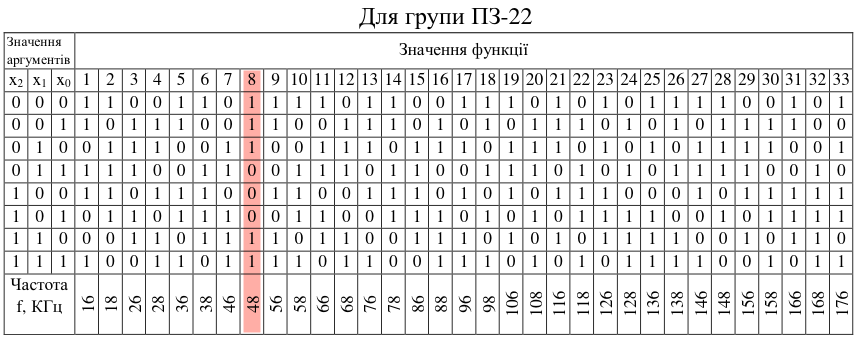
\includegraphics[scale=0.75]{v}
	\end{figure}	

	\section*{Теоретичні відомості}
	Логічний елемент - це електронне коло, що реалізує одну з елементарних логічних операцій.
	
	Логічна операція є елементарною якщо її можна описати булевою функцією одного або двох аргументів.
	
	Основні логічні операції, визначені аксіомами алгебри логіки можна реалізувати основними логічними елементами - інвертор (НЕ/NOT), диз'юнктор (АБО/OR), кон'юнктор (І/AND).
	
	З принципу двоїстості слідує, що будь-яку логічну функцію можна задати лише двома основними операціями: АБО та НЕ або ж І та НЕ.
	На практиці замість елементів АБО та НЕ використовують елемент Пірса, що є їх поєднанням, а замість елементів І та НЕ використовують елемент Шеффера.
	
	Proteus - це САПР для проектування найрізноманітніших електронних пристроїв.
	Інтерфейс програми є дуже подібним до класичного графічного інтерфейсу найбільш поширених програм.
	
	\section*{Хід роботи}
	\begingroup
	\setlength{\belowdisplayskip}{-15pt}
	\setlength{\abovedisplayskip}{0pt}
	\subsection*{Період цифрового сигналу}
	\begin{large}
		\begin{gather}
			T=\frac{1}{f};\hspace{22mm}T=\frac{1}{48\text{кГц}}=\frac{1}{48000\text{Гц}}=0.0000208\text{с}\nonumber
		\end{gather}
	\end{large}
	\subsection*{Кінцевий момент часу моделювання}
	\begin{large}
		\begin{gather}
			t\text{к}=2T;\hspace{22mm}t\text{к}=2\cdot0.0000208=0.0000416\text{с}\nonumber
		\end{gather}
	\end{large}
	\subsection*{ДДНФ заданої функції}
	\begin{large}
		\begin{gather}
			F_1=\overline{x_2}\overline{x_1}\overline{x_0}+\overline{x_2}\overline{x_1}x_0+\overline{x_2}x_1\overline{x_0}+x_2x_1\overline{x_0}+x_2x_1x_0	\nonumber
		\end{gather}
	\end{large}

	\subsection*{ДКНФ заданої функції}
	\begin{large}
		\begin{gather}
			F_2=(x_2+\overline{x_1}+\overline{x_0})(\overline{x_2}+x_1+x_0)(\overline{x_2}+x_1+\overline{x_0})\nonumber
		\end{gather}
	\end{large}
	\endgroup
	
	\begin{figure}[H]
		\centering
		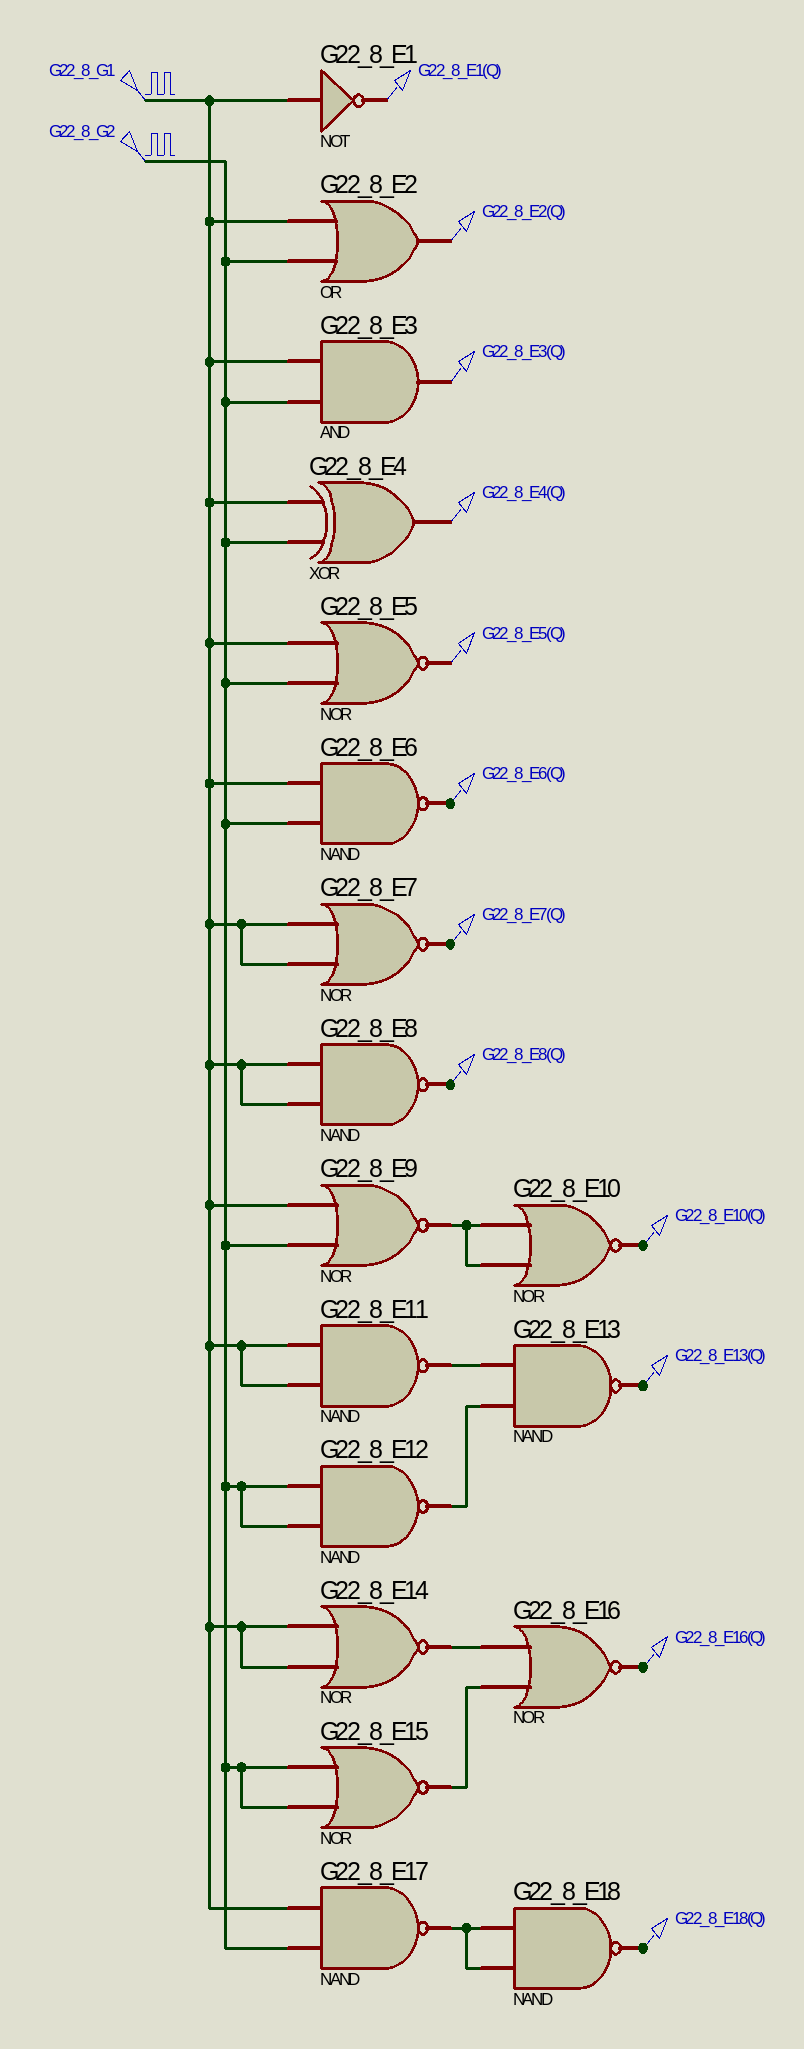
\includegraphics[scale=0.34]{s1}	
		\caption{Схема 1}
	\end{figure}
\vspace{-2mm}
	\begin{figure}[H]
		\centering
		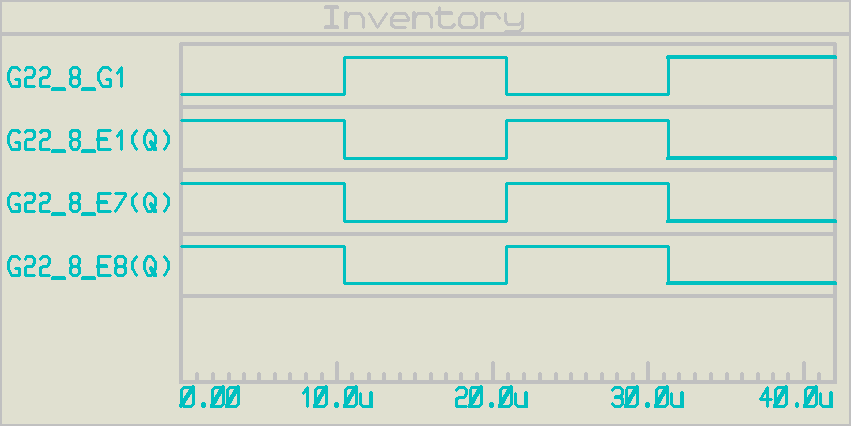
\includegraphics[scale=0.57]{g1}
		\caption{Графік "Inventory"}
	\end{figure}
	\begin{figure}[H]
		\centering
		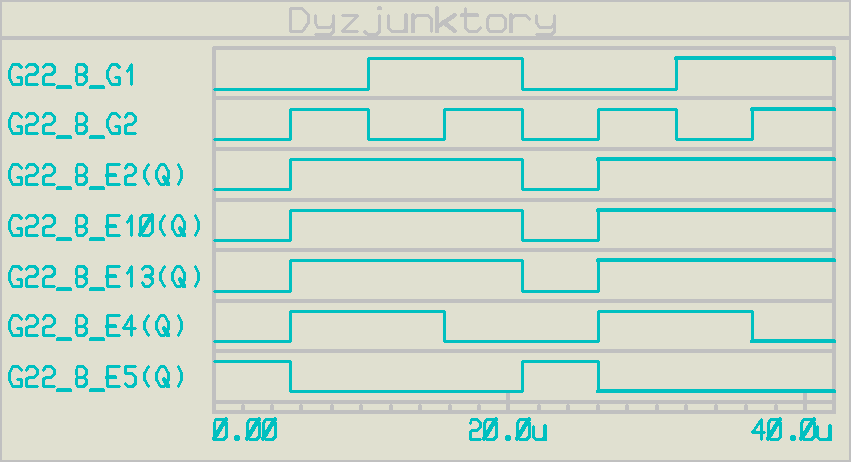
\includegraphics[scale=0.57]{g2}
		\caption{Графік "Dyzjunktory"}
	\end{figure}
	\begin{figure}[H]
		\centering
		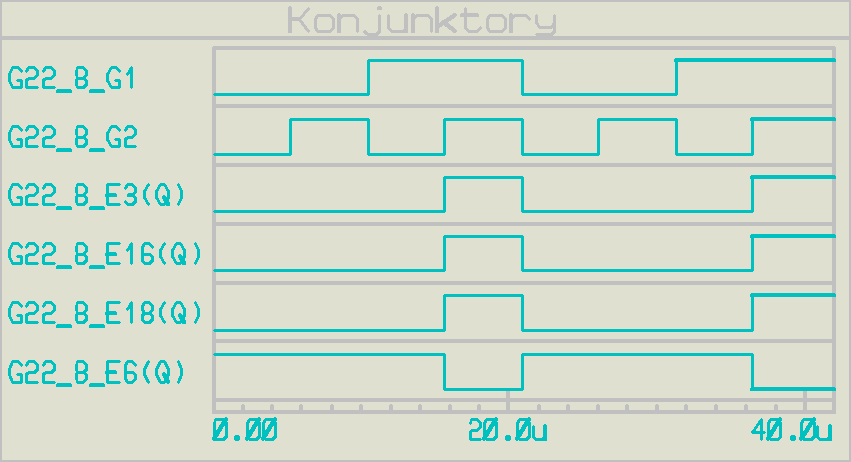
\includegraphics[scale=0.57]{g3}
		\caption{Графік "Konjunktory"}
	\end{figure}

	\begin{figure}[H]
		\centering
		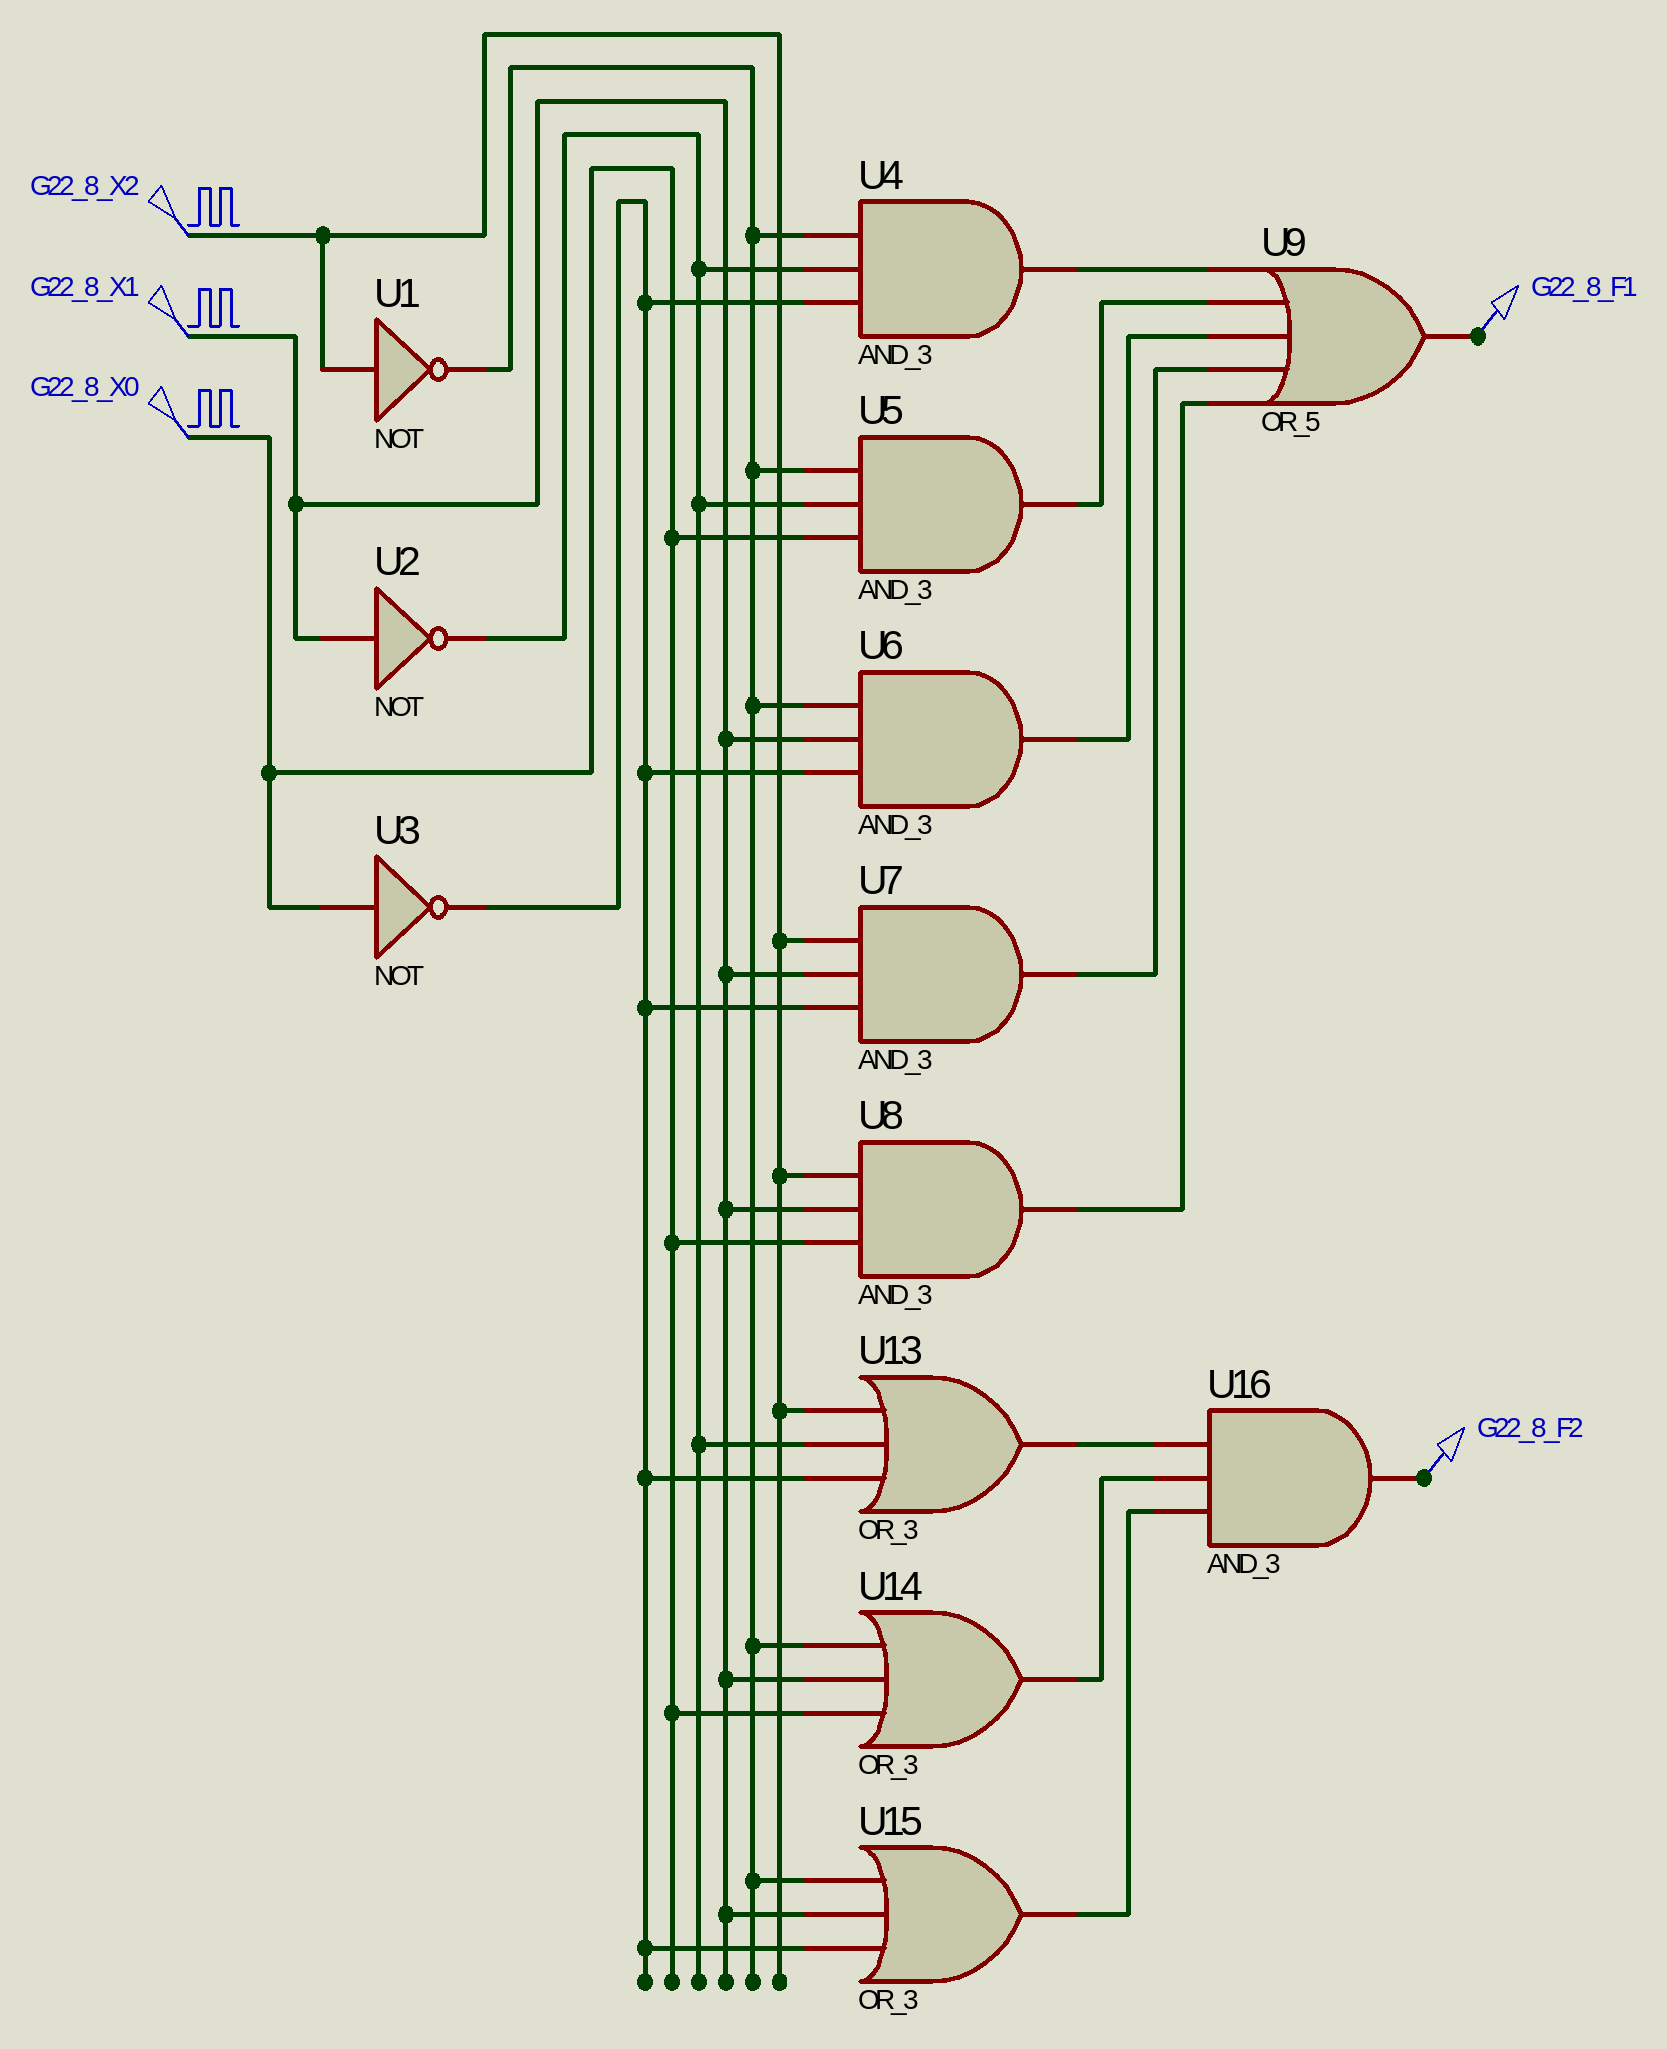
\includegraphics[scale=0.29]{s2}	
		\caption{Схема 2}
	\end{figure}
	\begin{figure}[H]
		\centering
		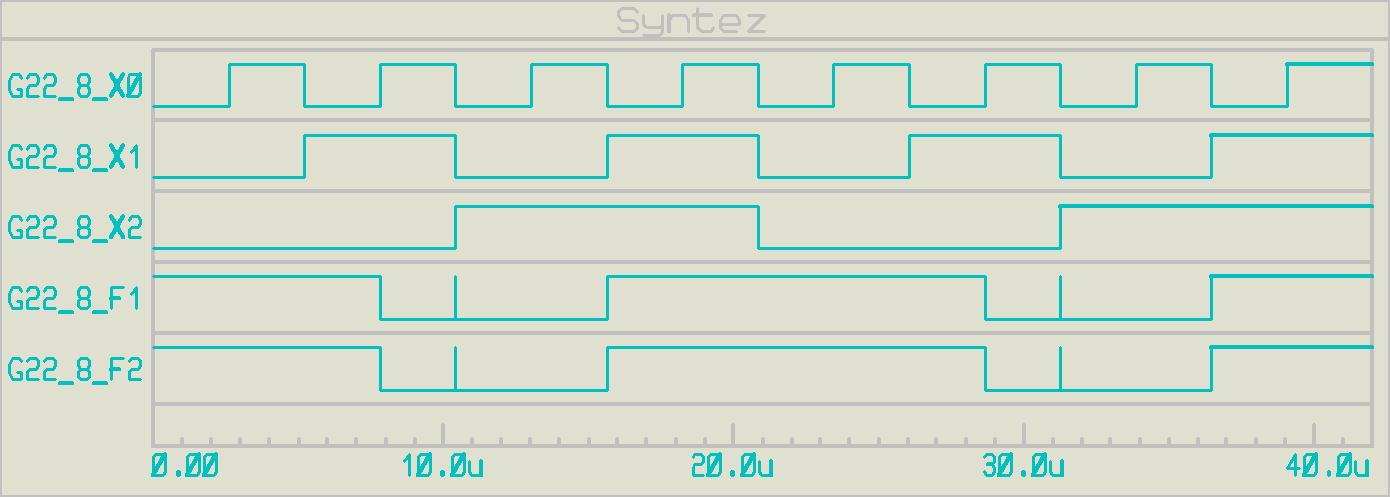
\includegraphics[scale=0.35]{g4}	
		\caption{Графік "Syntez"}
	\end{figure}	

	На графіку "Syntez" криві $G22\_8\_F1$ та $G22\_8\_F2$ повністню співпадають, тому можна зробити висновок, що ДДНФ та ДКНФ мають один результат при поданні логічної функції.

	\section*{Висновки}
	Під час виконання лабораторної роботи я навчився моделювати логічні елементи та схеми в середовищі системи програм Proteus; закріпив вміння складати за таблицею істиності логічні функції в досконалій диз'юнктивній та кон'юнктивній нормальній формі; синтезував прості схеми ДДНФ та ДКНФ логічної функції. Змоделював графіки цих функцій, що співпадають, тому можна зробити висновок, що моделювання виконано правильно.
	    
\end{normalsize}
\end{document}
